\documentclass[a4paper,12pt]{article}

\newcommand{\CRTdocFormat}{Пояснительная записка}
\usepackage{styledoc19}

\newcommand{\CRTdocnumMID}{ПЗ 01-1}
\usepackage{CRTconfig}

% \usepackage{refcheck}
\usepackage{tikz}

\usepackage{environ}
\usepackage{ltablex}
\keepXColumns

\NewEnviron{CRTtable}[2]{
  \noindent\begin{tabularx}{\textwidth}{#2}
    \caption{#1}\\
    \hline
    \BODY
  \end{tabularx}
}

\NewEnviron{CRTfieldtableC}[1]{
  \noindent\begin{tabularx}{\textwidth}{|l|l|X|}
    \caption{Описание полей класса #1}\label{tabfield#1}
    \\\hline \multicolumn{3}{|l|}{\textbf{Поля}}
    \\\hline \textbf{Имя} & \textbf{Тип} & \textbf{Назначение} \\\hline
    \endfirsthead
    \caption*{Продолжение таблицы \ref{tabfield#1}}
    \\\hline \multicolumn{3}{|l|}{\textbf{Поля}}
    \\\hline \textbf{Имя} & \textbf{Тип} & \textbf{Назначение} \\\hline
    \endhead
    \BODY
  \end{tabularx}
}

\NewEnviron{CRTmethodtableC}[2]{
  \noindent\begin{tabularx}{\textwidth}{|l|l|p{\widthof{#2}}|X|}
    \caption{Описание методов класса #1}\label{tabmethod#1}
    \\\hline \multicolumn{4}{|l|}{\textbf{Методы}}
    \\\hline \textbf{Имя} & \textbf{Тип} & \textbf{Аргументы} & \textbf{Назначение} \\\hline
    \endfirsthead
    \caption*{Продолжение таблицы \ref{tabmethod#1}}
    \\\hline \multicolumn{4}{|l|}{\textbf{Методы}}
    \\\hline \textbf{Имя} & \textbf{Тип} & \textbf{Аргументы} & \textbf{Назначение}
    \endhead
    \BODY
  \end{tabularx}
}

\makeatletter
\newcommand\subsubsubsection{\@startsection{paragraph}{4}{\z@}%
            {-2.5ex\@plus -1ex \@minus -.25ex}%
            {1.25ex \@plus .25ex}%
            {\normalfont\normalsize\bfseries}}
\makeatother
\setcounter{secnumdepth}{4} % how many sectioning levels to assign numbers to
\setcounter{tocdepth}{4}    % how many sectioning levels to show in ToC

\begin{document} % конец преамбулы, начало документа
  \CRTpreamble

  \section{Введение}
  \subsection{Наименование программы}
  <<\CRTname>>

  \subsection{Документы, на основании которых ведется разработка}
  Основанием для разработки является учебный план подготовки бакалавров по направлению 09.03.04 <<Программная инженерия>> и утвержденная академическим руководителем тема курсового проекта.

  \newpage
  \section{Назначение и область применения}
  \subsection{Назначение программы}
  \subsubsection{Функциональное назначение}
  Разрабатываемое приложение <<\CRTname>> предназначено для создания снимка экрана рабочей зоны компьютера и для дальнейшей работы и обработки таких снимков с возможностью добавления текста и графических набросков на основе алгоритмов математических кривых Безье.
  \subsubsection{Эксплуатационное назначение}
  Программа предназначена для бытового пользователя на компьютерах с операционной системой Windows и Linux.
  \subsection{Область применения}
  Программа используется в повседневной жизни, когда требуется создание и сохранение снимка экрана с возможностью дальнейшего редактирования, включая обрезание, создание набросков и добавление текста.
  % Возможность скрывать лишнюю информацию на скриншотах прямоугольниками

  \newpage
  \section{Технические характеристики}
  \subsection{Постановка задачи на разработку программы}
  Программа разработана в соответствии с техническим заданием <<\CRTname>>.

  Для разработки данного проекта были выделены следующий задачи:
  \begin{enumerate}
    \item Разработка алгоритма для построения кривой Безье по заданному набору точек.
    \item Разработка алгоритма для разбиения кривой Безье на множество прямых сегментов.
    \item Разработка алгоритма для разбиения ломаной линии определённой толщины на множество треугольников.
    \item Разработка простейшего кроссплатформенного интерфейса, для работы с буфером обмена изображений.
    \item Разработка пользовательского интерфейса.
  \end{enumerate}

  \subsection{Описание применяемых технологических методов}
  Программа представляет собой кроссплатформенное десктоп приложение,
  написанное на языке программирования C с использованием технологии OpenGL\cite{opengl}.
  Для открытия окон используется библиотеки GLFW\cite{glfw} и raylib\cite{raylib}.

  \subsubsection{Описание общей схемы работы приложения}
  \begin{enumerate}
    \item При запуске программы, из буфера обмена подгружается изображение, или, если его там нет, пользователю предлагается сделать скриншот.
    \item Пользователю предоставляется возможность редактирования изображения.
    \begin{itemize}
      \item Редактирование осуществляется путём добавления на изображения различных элементов (см. \autoref{tabfieldDrawable}).
      \item Элементы начинают свой жизненный цикл активными.
      Пользователь может взаимодействовать только с активными элементами.
      Только один элемент может быть активен в некоторый момент времени,
      так как новые элементы можно добавлять только когда активных нет (см. \autoref{tabfieldCanvas}).
      \item У каждого типа элементов свой цвет по умолчанию, но пользователь может его менять.
    \end{itemize}
    \item При закрытии программы отредактированное изображение сохраняется обратно в буфер обмена.
  \end{enumerate}

  \subsubsection{Описание алгоритма построения кривой Безье}
  \label{sec:curvealgo}
  Для реализации алгоритма построения кривых Безье за основу был взят рекурсивный алгоритм из книги Graphics Gems\cite{algo}.

  На вход он получает последовательность точек и единичные касательные вектора на концах.
  Когда этот алгоритм используется для рисования мышкой, массив точек строится как позиция мышки на каждом кадре, где она переместилась,
  а касательные вектора считаются как нормированная разность двух соседних точек.
  В результате у нас получается последовательность кривых Безье третьего порядка (сплайн), в которой нет разрывов и перегибов.

  Поскольку нам нужно получить непрерывную кривую, каждая кубическая кривая Безье определяется только двумя, а не восемью параметрами.
  Это нам позволяет минимизировать среднеквадратическую ошибку решив систему из двух линейных уравнений.
  Но для нахождения среднеквадратической ошибки нужно знать расстояние от произвольной точки до кривой Безье,
  а это дорогостоящая операция.
  Вместо нахождения ближайшей точки на кривой Безье можно взять предположительное значение параметра $t$,
  основываясь на длине хорд\cite{chordlength}.

  Теперь, чтобы получить среднеквадратическую ошибку $S$, нужно сложить расстояния от каждой исходной точки $\mathbf{V}_i$ до точки на кривой Безье, соответствующей предположительному значение параметра $t_i$.
  Точка на кривой Безье находится также как и в разделе \ref{sec:wikialgo}.
  $$ S = \sum_{i=0}^n \left(\vphantom{\frac{1}{2}}\mathbf{V}_i-\mathbf{B}(t_i)\right)^2 $$

  Контрольные точки $\mathbf{P}_0$ и $\mathbf{P}_3$ зафиксированы как $\mathbf{V}_0$ и $\mathbf{V}_n$,
  а $\mathbf{P}_1$ и $\mathbf{P}_2$ лежат на касательных векторах и отдаленны от $\mathbf{P}_0$ и $\mathbf{P}_3$ на $\alpha_1$ и $\alpha_2$ соответственно.
  Их можно найти прировняв частные производные $S$ к нулю.
  $$\frac{\partial S}{\partial \alpha_1} = 0$$
  $$\frac{\partial S}{\partial \alpha_2} = 0$$

  \begin{enumerate}
    \item Строим кривую Безье минимизируя среднеквадратическую ошибку.
    \item Если не хватает точности, мы делаем до четырёх итераций параметризации $t_i$ методом Ньютона\cite{NewtonRaphson}.
    \item Если точности до сих пор не хватает, то мы разделяем набор точек на две части и запускаем алгоритм рекурсивно на каждой из них.
  \end{enumerate}

  \subsubsection{Описание алгоритма разбиения кривой Безье на ломаную линию}
  \label{sec:wikialgo}
  Сплайн, полученный алгоритмом, который описан в разделе \ref{sec:curvealgo}, состоит исключительно из кубических кривых Безье.
  Кривые Безье определяются параметрически, поэтому, чтобы получить ломаную линию, приближённую к такому сплайну,
  надо просто посчитать координаты некоторого количества равномерно распределённых точек на каждой кривой Безье.

  По определению кривая Безье порядка $n$ строится через $\frac{n(n+1)}{2}-1$ вспомогательных точек.
  Параметр $t$ определяет где именно на отрезке от $P_i$ до $P_{i+1}$ находится $Q_i$, и так для всех остальных вспомогательных точек.
  В случае кубических кривых Безье будет $5$ вспомогательных точек:
  $Q_0$, $Q_1$, $Q_2$, $R_0 $ и $R_1$ \CRTfigref{wikicurve}{Построение кривой Безье третьего порядка}.

  Отношение отрезков получается такое:
  $$ \frac{P_{0}Q_{0}}{P_{0}P_{1}}=\frac{Q_{1}P_{1}}{P_{1}P_{2}}=\frac{BR_{0}}{R_{1}R_{0}} = t $$

  Это можно упростить и получить полиномиальную формулу:
  $$ \mathbf{B}(t) = (1-t)^3\mathbf{P}_0+3(1-t)^2t\mathbf{P}_1+3(1-t)t^2\mathbf{P}_2+t^3\mathbf{P}_3 $$

  \subsubsection{Описание алгоритма соединения двух сегментов ломаной линии}
  \label{sec:linejoin}
  Ломаная линия задана как последовательность точек (на \autoref{fig:linejoin} отмечены красным).
  Алгоритм находит точки, из которых можно построить ленту треугольников (на \autoref{fig:linejoin} отмечены зелёным).

  Для каждой точки и её двух соседей:
  \begin{enumerate}
    \item Находим два единичных направляющих вектора (на \autoref{fig:linejoin} отмечены синим), складываем их и нормируем.
    \item Делим получившийся вектор на его скалярное произведение на один из направляющих векторов. Если он получается длиннее $10$, ограничиваем его длину. Такое ограничение нужно, для того чтобы, когда два отрезка линии встречаются под очень острым углом, точка соединения не могла выходить далеко за пределы толщины линии\cite{miterlimit}.
    \item Вычитаем и прибавляем полученный вектор, домноженный на желаемую толщину линии, к центральной точке. Две полученные точки идут к нам в ответ.
  \end{enumerate}

  \begin{figure}[h!]
    \centering
    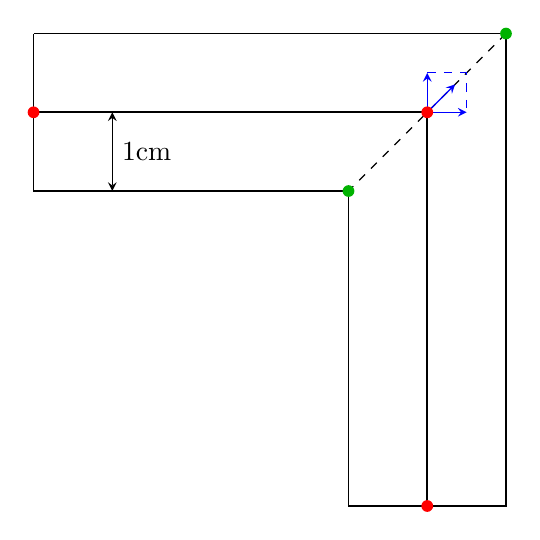
\begin{tikzpicture}[x=1cm,y=1cm]
      \draw[thick] (-5,0)--(0,0)--(0,-5);
      \draw (-5,1)--(1,1)--(1,-5)--(-1,-5)--(-1,-1)--(-5,-1)--(-5,1);
      \draw[dashed] (1,1)--(-1,-1);

      \draw[dashed, blue] (0,.5)--(.5,.5)--(.5,0);
      \draw[-stealth, blue] (0,0)--(0,.5);
      \draw[-stealth, blue] (0,0)--(.5,0);
      \draw[-stealth, blue] (0,0)--(.3535,.3535);

      \draw[stealth-stealth] (-4,-1)--(-4,0);
      \node[right] at (-4,-.5) {1cm};

      \node at (-5,0) [circle,fill=red,inner sep=1.5pt]{};
      \node at (0,0) [circle,fill=red,inner sep=1.5pt]{};
      \node at (0,-5) [circle,fill=red,inner sep=1.5pt]{};
      \node at (1,1) [circle,fill=black!30!green,inner sep=1.5pt]{};
      \node at (-1,-1) [circle,fill=black!30!green,inner sep=1.5pt]{};
    \end{tikzpicture}
    \caption{Соединение двух линий}
    \label{fig:linejoin}
  \end{figure}

  % \subsubsection{Описание схемы функционирования программы}
  % \subsubsection{Возможные взаимодействия программы с другими программами}
  \subsection{Обоснование выбора алгоритма решения задачи}
  Сплайны из кубических кривых Безье используются, потому что они является стандартными в области компьютерной графики\cite{curves}.
  Конвертация этих сплайнов сначала в ломаные линии, а потом в ленты треугольников, это один из самых простых способов их отрисовки в OpenGL, ведь OpenGL напрямую поддерживает ленты треугольников\cite{triangleStrip}.

  Кодировка UTF-8, в отличие от других Unicode кодировок (UTF-16 и UTF-32),
  совместима со стандартной библиотекой языка программирования C, которая работает с нуль-терминированными строками.
  Это также позволяет не отличать ASCII и Unicode строки в исходном коде.

  Алгоритм, описанный в разделе \ref{sec:linejoin}, нужен чтобы на кривой точно заполнялись все пиксели.
  Он хорош тем, что прост в реализации и всегда генерирует ленту треугольников,
  количество точек в которой ровно в два раза больше чем в исходной ломаной линии.

  \subsection{Описание и обоснование выбора метода организации входных и выходных данных}
  \subsubsection{Описание метода организации входных и выходных данных}
  Входные и выходные данные, согласно техническому заданию, являются изображением,
  которое находится, либо в буфере обмена, либо в файле в формате PNG.
  В операционной системе Windows буфер обмена хранит изображения в формате BITMAP\cite{clipboardFormats},
  а в Unix-подобных системах они хранятся в формате PNG.

  \subsubsection{Обоснование выбора метода организации входных и выходных данных}
  Выходные данные организованы в формате PNG в силу требований технического задания.
  Также использование любого другого формата растровых изображений было бы не логично,
  так как JPEG сжимает изображение с потерями и не поддерживает прозрачность, а более сложные форматы могут не поддерживается.

  \subsection{Описание и обоснование выбора состава технических и программных средств}
  \subsubsection{Состав технических и программных средств}
  Состав технических средств, необходимых для работы системы:
  \begin{enumerate}
    \item Процессор архитектуры x86 или x64 с частотой не менее 1 ГГц;
    \item Не менее 1 ГБ ОЗУ;
    \item Не менее 5 МБ свободного места на жестком диске;
    \item Поддержка графических интерфейсов OpenGL или Vulkan;
    \item Одна из нижеперечисленных операционных систем:
    \begin{itemize}
      \item Unix-подобная операционная система с оконной системой X11;
      \item Windows XP или более поздняя версия операционной системы (32-разрядные или 64-разрядные).
    \end{itemize}
  \end{enumerate}

  \subsubsection{Обоснование выбора состава технических средств}
  Состав технических средств был выбран согласно составу технических средств для библиотеки GLFW.

  \newpage
  \section{Технико-экономические показатели}
  \subsection{Ориентировочная экономическая эффективность}
  Для данного проекта подсчет экономической эффективности не предусмотрен.

  \subsection{Предполагаемая потребность}
  Предполагается, что разработанной программой будет пользоваться среднестатистический пользователь персонального компьютера или ноутбука, который желает сделать изображение рабочей зоны экрана.
  % \section{Экономические преимущества по сравнению с отечественными и зарубежными аналогами}

  \begin{CRTbibliography}
    \bibitem{algo}
    Glassner, Andrew. Graphics Gems. Academic Press, 1990, pp. 612-626.
    //URL: \url{http://inis.jinr.ru/sl/vol1/CMC/Graphics_Gems_1,ed_A.Glassner.pdf}
    % как оформить цитату на http://inis.jinr.ru/sl/vol1/CMC/Graphics_Gems_1,ed_A.Glassner.pdf страница 626 в библиографии?

    \bibitem{NewtonRaphson}
    Статья <<Newton's method>> Wikipedia.org
    //URL: \url{https://en.wikipedia.org/wiki/Newton%27s_method}
    (Дата обращения: 11.05.2021, режим доступа: свободный)

    \bibitem{curves}
    Статья <<Composite Bézier curve>> Wikipedia.org
    //URL: \url{https://en.wikipedia.org/wiki/Composite_B%C3%A9zier_curve}
    (Дата обращения: 11.05.2021, режим доступа: свободный)

    \bibitem{triangleStrip}
    Статья <<Triangle strip>> Wikipedia.org
    //URL: \url{https://en.wikipedia.org/wiki/Triangle_strip}
    (Дата обращения: 11.05.2021, режим доступа: свободный)

    \bibitem{chordlength}
    Статья <<The Chord Length Method>> pages.mtu.edu
    //URL: \url{https://pages.mtu.edu/~shene/COURSES/cs3621/NOTES/INT-APP/PARA-chord-length.html}
    (Дата обращения: 11.05.2021, режим доступа: свободный)

    \bibitem{raylib}
    Документация библиотеки raylib [Электронный ресурс] //URL: \url{http://raylib.com/}
    (Дата обращения: 11.05.2021, режим доступа: свободный)

    \bibitem{opengl}
    Документация OpenGL [Электронный ресурс] //URL: \url{https://www.opengl.org/}
    (Дата обращения: 11.05.2021, режим доступа: свободный)

    \bibitem{glfw}
    Документация GLFW [Электронный ресурс] //URL: \url{https://www.glfw.org/}
    (Дата обращения: 11.05.2021, режим доступа: свободный)

    \bibitem{clipboardFormats}
    Документация Microsoft Clipboard Formats [Электронный ресурс]
    //URL: \url{https://docs.microsoft.com/en-us/windows/win32/dataxchg/clipboard-formats}
    (Дата обращения: 11.05.2021, режим доступа: свободный)

    \bibitem{miterlimit}
    Документация SVG stroke-miterlimit [Электронный ресурс]
    //URL: \url{https://developer.mozilla.org/en-US/docs/Web/SVG/Attribute/stroke-miterlimit}
    (Дата обращения: 11.05.2021, режим доступа: свободный)
  \end{CRTbibliography}

  \CRTterminology

  \addition{Описание и функциональное назначение классов}
  \label{sec:classtable}
  \begin{CRTtable}{Классы проекта}{|l|X|}
    \textbf{Класс} & \textbf{Назначение}
    \\\hline Drawable & Интерфейс, который реализуют все элементы добавляемые пользователем на изображение
    \\\hline Canvas & Отрисовка редактируемого изображения и добавление на него элементов
    \\\hline Screenshot & Работа с буфером обмена и взятие скриншотов
    \\\hline Editor & Логика интерфейса главного окна
    \\\hline CropRectangle & Прямоугольник. Может быть закрашенным или обрезать изображение. Реализует интерфейс Drawable
    \\\hline DrawableLine & Линия, нарисованная от руки. Реализует интерфейс Drawable
    \\\hline FloatingImage & Картинка, добавленная на изображение с помощью перетаскивания. Реализует интерфейс Drawable
    \\\hline Textbox & Текстовое поле. Реализует интерфейс Drawable
    \\\hline
  \end{CRTtable}

  \addition{Описание и функциональное назначение методов и полей}
  \label{sec:tables}

  \begin{CRTfieldtableC}{Drawable}
    self & void* & Указатель на реализацию \\\hline
    name & char* & Название типа, который реализует этот интерфейс \\\hline
    update & UpdateMethod & Реализация метода Update \\\hline
    draw & Method & Реализация метода Draw \\\hline
    delete & Method & Реализация метода Delete \\\hline
    move & MoveMethod & Реализация метода Move \\\hline
    setColor & ColorMethod & Реализация метода SetColor \\\hline
  \end{CRTfieldtableC}

  \begin{CRTmethodtableC}{Drawable}{FrameworkElement}
    Update & bool & Drawable* & Даёт элементу возможность обновится и прочитать позицию мышки и состояние клавиатуры \\\hline
    Draw & void & Drawable* & Отображает элемент на экране \\\hline
    Delete & void & Drawable* & Удаляет элемент и освобождает память \\\hline
    Move & void & Drawable*, Vector2 & Передвигает элемент \\\hline
    SetColor & void & Drawable*, Color & Меняет цвет элемента \\\hline
  \end{CRTmethodtableC}

  \begin{CRTfieldtableC}{Canvas}
    scale & float & Масштаб изображения \\\hline
    pos & Vector2 & Позиция изображения на экране \\\hline
    texture & Texture & Текстура, в которой хранится изначальное немодифицированное изображение \\\hline
    screenshot & Screenshot & Вспомогательный объект для взятие скриншотов \\\hline
    scaleIndex & float & Индекс выбранного масштаба \\\hline
    scrollAccumulator & float & Аккумулятор дробных движений колёсика мышки \\\hline
    nearestNeighborToggle & bool & Режим масштабирования изображения \\\hline
    scheduledReload & bool & Нужно ли обновлять состояние на следующий кадр \\\hline
    transparencyTexture & Texture & Текстура прозрачного фона \\\hline
    screenWidth & float & Ширина экрана \\\hline
    screenHeight & float & Высота экрана \\\hline
    prevMousePos & Vector2 & Предыдущая позиция мышки \\\hline
    marginTopLeft & Vector2 & Размер полей в верхнем левом углу \\\hline
    marginBottomRight & Vector2 & Размер полей в нижнем правом углу \\\hline
    color & Color & Цвет новых добавленных элементов \\\hline
    drawables & Drawable* & Список элементов добавленных пользователем на изображение \\\hline
    isActive & bool & Активен ли последний элемент \\\hline
  \end{CRTfieldtableC}

  \begin{CRTmethodtableC}{Canvas}{Canvas*, Drawable}
    recenter & void & Canvas* & Помещает изображение на центр экрана \\\hline
    rescale & void & Canvas* & Подбирает оптимальный масштаб изображения \\\hline
    popDrawable & bool & Canvas* & Удаляет последний добавленный элемент \\\hline
    updateSize & void & Canvas* & Обновляет размер экрана \\\hline
    reload & void & Canvas*, bool & Подгружает новое изображение из буфера обмена \\\hline
    zoom & void & Canvas*, int & Изменяет масштаб \\\hline
    updateDrawable & void & Canvas* & Обновляет активный элемент \\\hline
    takeScreenshot & void & Canvas* & Делает скриншот и подгружает его как новое изображение \\\hline
    keyboardShortcuts & void & Canvas* & Проверяет клавиши быстрого доступа \\\hline
    copy & bool & Canvas*, char* & Сохраняет отредактированное изображение в буфера обмена или в файл \\\hline
    addDrawable & void & Canvas*, Drawable & Добавляет новый элемент \\\hline
    Update & void & Canvas* & Редактирует изображение \\\hline
    Draw & void & Canvas* & Отображает изображение и все добавленные на него элементы на экране \\\hline
    loadImage & bool & Canvas*, char* & Подгружает новое изображение из файла \\\hline
    SetColor & void & Canvas*, Color & Меняет цвет активного элемента и новых элементов \\\hline
  \end{CRTmethodtableC}

  \begin{CRTfieldtableC}{Screenshot}
    image & Image & Временный буфер для хранения изображений \\\hline
    texture & Texture & Текстура, в которой хранится текущие изображение \\\hline
    renderTexture & RenderTexture & Текстура, в которую будет везтись отрисовка, при сохранении изображения \\\hline
    width & int & Ширина буфера \\\hline
    height & int & Высота буфера \\\hline
  \end{CRTfieldtableC}

  \begin{CRTmethodtableC}{Screenshot}{\textbf{Аргументы}}
    getImageFromClipboard & Image &  & Достаёт изображение из буфера обмена \\\hline
    putImageToClipboard & bool & Image & Помещает изображение в буфера обмена \\\hline
    takeScreenshot & bool &  & Делает скриншот \\\hline
    waitEvents & void &  & Приостанавливает работу программы пока пользователь ничего не делает  \\\hline
    setImage & bool & Screenshot*, Image & Копирует новое изображение в буфер \\\hline
    update & bool & Screenshot* & Подгружает изображение из буфера обмена \\\hline
    begin & void & Screenshot* & Начинает перенаправление графики в буферную текстуру \\\hline
    end & bool & Screenshot*, char* & Заканчивает перенаправление графики в буферную текстуру и сохраняет результат в файл или буфер обмена \\\hline
    Delete & void & Screenshot* & Удаляет буфер и освобождает память \\\hline
  \end{CRTmethodtableC}

  \begin{CRTfieldtableC}{Editor}
    canvas & Canvas & Редактируемое изображение \\\hline
    filename & char* & Имя файла, который мы редактируем. NULL если мы редактируем буфер обмена \\\hline
    mode & UiMode & Режим пользовательского интерфейса \\\hline
    isUiHidden & bool & Спрятан ли пользовательский интерфейс \\\hline
    clickableCursor & bool & Определяет находится ли курсор мышки на кнопке \\\hline
    inputField & Textbox & Текстовое поле для ввода имени файла \\\hline
    ioError & bool & Была ли ошибка при последней попытке открыть файл \\\hline
    buttonRect & Rectangle & Прямоугольник кнопки \\\hline
  \end{CRTfieldtableC}

  \begin{CRTmethodtableC}{Editor}{FrameworkElement}
    setMode & void & Editor*, UiMode & Изменяет режим пользовательского интерфейса \\\hline
    toggleUi & void & Editor* & Прячет пользовательский интерфейс  \\\hline
    open & bool & Editor*, char* & Открывает файл \\\hline
    Draw & void & Editor* & Отображает пользовательский интерфейс \\\hline
    Update & void & Editor* & Обрабатывает действия пользователя \\\hline
  \end{CRTmethodtableC}

  \begin{CRTfieldtableC}{CropRectangle}
    parentCanvas & Canvas* & Указатель на Canvas, в который был добавлен этот элемент \\\hline
    point1 & Vector2 & Первый угол прямоугольника \\\hline
    point2 & Vector2 & Второй угол прямоугольника \\\hline
    hasFirstPoint & bool & Есть ли первая точка \\\hline
    isDone & bool & Закончил ли пользователь создание прямоугольника \\\hline
    isHollow & bool & Нужно ли закрашивать прямоугольник или только рисовать рамки \\\hline
    frameColor & Color & Цвет рамки и прямоугольника \\\hline
  \end{CRTfieldtableC}

  \begin{CRTmethodtableC}{CropRectangle}{CropRectangle*,}
    get & Rectangle & CropRectangle* & Возвращает правильно отформатированный прямоугольник, находя левый верхний угол, ширину и высоту \\\hline
    getSmall & Rectangle & CropRectangle* & Возвращает прямоугольник ограниченный размерами изображения \\\hline
    selfDestruct & void & CropRectangle* & Удаляет себя из списка добавленных элементов \\\hline
    crop & void & CropRectangle* & Обрезает изображения по границам этого прямоугольника \\\hline
    Draw & void & CropRectangle* & Отображает прямоугольник на экране. Реализация метода Draw из интерфейса Drawable \\\hline
    Update & bool & CropRectangle* & Обновляет позицию прямоугольника. Реализация метода Update из интерфейса Drawable \\\hline
    Delete & void & CropRectangle* & Удаляет прямоугольник и освобождает память. Реализация метода Delete из интерфейса Drawable \\\hline
    Move & void & CropRectangle*, Vector2 & Передвигает прямоугольник. Реализация метода Move из интерфейса Drawable \\\hline
    SetColor & void & CropRectangle*, Color & Меняет цвет прямоугольника. Реализация метода SetColor из интерфейса Drawable \\\hline
    New & Drawable & Canvas* & Создаёт новый CropRectangle и упаковывает его в интерфейс Drawable \\\hline
  \end{CRTmethodtableC}

  \begin{CRTfieldtableC}{DrawableLine}
    line & Vector2* & Список точек в линии \\\hline
    triangleStrip & Vector2* & Лента треугольников \\\hline
    triangleStripLength & int & Количество точек в ленте треугольников \\\hline
    error & float & Максимальное допустимое отклонение при построение кривой Безье \\\hline
    thickness & float & Толщина линии \\\hline
    subdivisions & int & Количество прямых сегментов, на которые будет разбита каждая кривая Безье \\\hline
    color & Color & Цвет линии \\\hline
  \end{CRTfieldtableC}

  \begin{CRTmethodtableC}{DrawableLine}{DrawableLine*,}
    \_init & void & DrawableLine* & Инициализирует все поля дефолтными значениями \\\hline
    add & void & DrawableLine*, Vector2 & Добавляет новую точки в конец линии \\\hline
    getTriangleStrip & Vector2* & DrawableLine* & Конвертирует линию в ленту треугольников \\\hline
    setOptions & bool & DrawableLine*, float, float, int, Color & Устанавливает параметры линии \\\hline
    drawDebug & void & DrawableLine* & Выводит на экран параметры линии \\\hline
    Draw & void & DrawableLine* & Отображает линию на экране. Реализация метода Draw из интерфейса Drawable \\\hline
    Update & bool & DrawableLine* & Обновляет линию, добавляя новую точки, если позиция мышки изменилась. Реализация метода Update из интерфейса Drawable \\\hline
    Delete & void & DrawableLine* & Удаляет картинку и освобождает память. Реализация метода Delete из интерфейса Drawable \\\hline
    Move & void & DrawableLine*, Vector2 & Передвигает картинку. Реализация метода Move из интерфейса Drawable \\\hline
    SetColor & void & DrawableLine*, Color & Меняет цвет рамки картинки. Реализация метода SetColor из интерфейса Drawable \\\hline
    New & Drawable &  & Создаёт новый DrawableLine и упаковывает его в интерфейс Drawable \\\hline
  \end{CRTmethodtableC}

  \begin{CRTfieldtableC}{FloatingImage}
    pos & Vector2 & Позиция картинки \\\hline
    texture & Texture & Текстура картинки \\\hline
    hasFirstPoint & bool & Есть ли первая точка \\\hline
    isDone & bool & Закончил ли пользователь перемещение картинки \\\hline
    nearestNeighborToggle & bool & Режим масштабирования картинки \\\hline
    scale & float & Масштаб картинки \\\hline
    frameColor & Color & Цвет рамки \\\hline
  \end{CRTfieldtableC}

  \begin{CRTmethodtableC}{FloatingImage}{FloatingImage*,}
    Draw & void & FloatingImage* & Отображает картинку на экране. Реализация метода Draw из интерфейса Drawable \\\hline
    Update & bool & FloatingImage* & Обновляет позицию картинки. Реализация метода Update из интерфейса Drawable \\\hline
    Delete & void & FloatingImage* & Удаляет картинку и освобождает память. Реализация метода Delete из интерфейса Drawable \\\hline
    Move & void & FloatingImage*, Vector2 & Передвигает картинку. Реализация метода Move из интерфейса Drawable \\\hline
    SetColor & void & FloatingImage*, Color & Меняет цвет рамки картинки. Реализация метода SetColor из интерфейса Drawable \\\hline
    New & Drawable & char* & Создаёт новый FloatingImage и упаковывает его в интерфейс Drawable \\\hline
  \end{CRTmethodtableC}

  \begin{CRTfieldtableC}{Textbox}
    text & char* & Текст в UTF-8. Один символ может кодироваться несколькими байтами \\\hline
    cursorPos & int & Позиция курсора, то есть индекс первого байта после него \\\hline
    pos & Vector2 & Позиция текстового поля на экране \\\hline
    cursorColor & Color & Цвет курсора \\\hline
    textColor & Color & Цвет текста \\\hline
    fontSize & int & Размер шрифта \\\hline
    font & Font & Шрифт \\\hline
    showCursor & bool & Надо ли нам показывать курсор \\\hline
    thickCursor & bool & Будет ли курсор жирным или тонким \\\hline
  \end{CRTfieldtableC}

  \begin{CRTmethodtableC}{Textbox}{\textbf{Аргументы}}
    IsKeyTyped & bool & int & Проверяет была ли нажата в этот кадр клавиши, но, в отличие от IsKeyPressed, повторяется при зажатие \\\hline
    init & void & Textbox* & Инициализирует все поля дефолтными значениями \\\hline
    \_del & void & Textbox*, int & Удаляет $n$ байтов после курсора \\\hline
    \_ins & char* & Textbox*, int & Добавляет $n$ байтов перед курсором и возвращает указатель на первый из них \\\hline
    moveCursor & void & Textbox*, bool, bool & Передвигает курсор либо на один символ либо на одно слово \\\hline
    backspace & void & Textbox*, bool, bool & Удаляет последний напечатанный символ или слово \\\hline
    addCharacter & void & Textbox*, int & Добавляет символ на позиции курсора \\\hline
    addText & void & Textbox*, char* & Добавляет строку на позиции курсора \\\hline
    measureText & Vector2 & Textbox* & Измеряет длину текста в пикселях \\\hline
    partialMeasureText & Vector2 & Textbox* & Находит позицию курсора в пикселях \\\hline
    Draw & void & Textbox* & Отображает текстовое поле на экране. Реализация метода Draw из интерфейса Drawable \\\hline
    Update & bool & Textbox* & Обновляет позицию текстового поля и добавляет напечатанные символы. Реализация метода Update из интерфейса Drawable \\\hline
    Delete & void & Textbox* & Удаляет текстовое поле и освобождает память. Реализация метода Delete из интерфейса Drawable \\\hline
    Move & void & Textbox*, Vector2 & Передвигает текстовое поле. Реализация метода Move из интерфейса Drawable \\\hline
    SetColor & void & Textbox*, Color & Меняет цвет текста. Реализация метода SetColor из интерфейса Drawable \\\hline
    New & Drawable &  & Создаёт новый Textbox и упаковывает его в интерфейс Drawable \\\hline
  \end{CRTmethodtableC}

  \CRTlistRegistration
\end{document} % конец документа
